\documentclass{article}

\usepackage{graphicx}
\usepackage{tikz}
\usepackage{tikzsymbols}
\usetikzlibrary{calc,patterns,shapes.geometric}
\pagestyle{empty}
\usepackage[margin=0pt]{geometry}
\geometry{papersize={14in,12in}}

\def\centerarc[#1](#2)(#3:#4:#5){\draw[#1] ($(#2)+({#5*cos(#3)},{#5*sin(#3)})$) arc (#3:#4:#5);}

\begin{document}
	\begin{figure}
		\centering
		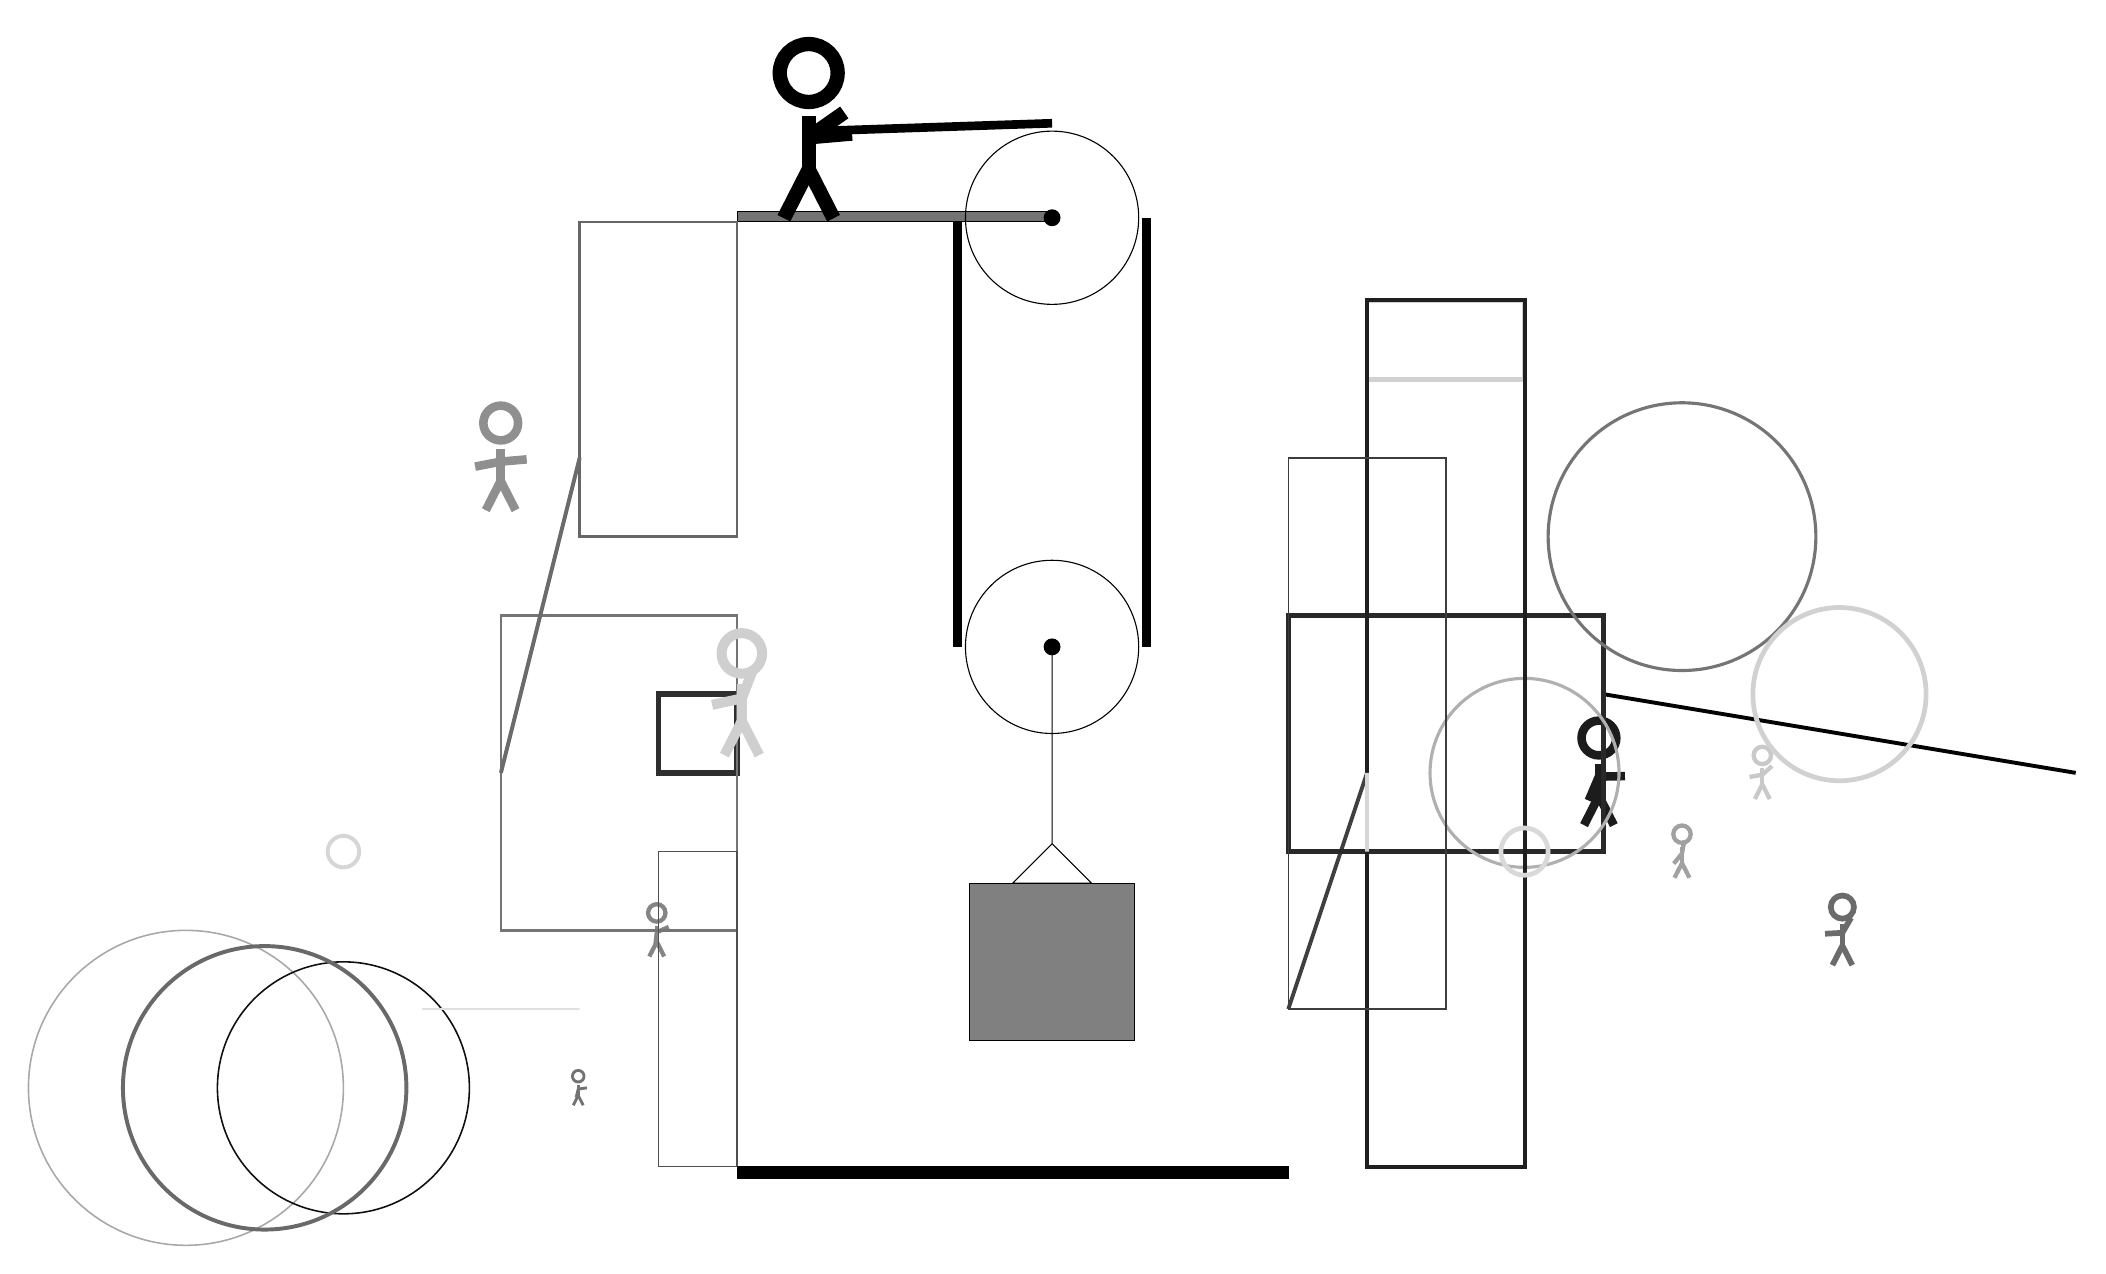
\begin{tikzpicture}
			%%%%% START %%%%%
			
			\draw[fill=black!55] (-2, 9) rectangle (2, 9.125);
			
			\draw (2, 3.6) circle (1.1);
			\draw[fill=black] (2, 3.6) circle (0.1);
			
			\draw (2, 9.05) circle (1.1);
			\draw[fill=black] (2, 9.05) circle (0.1);
			
			\draw [line width=0.2mm, color=black!34](-9, -2) circle (2.0);
			
			\node[line width=0.7mm, color=black!44] at (-5, 6) {\Strichmaxerl[6][11][5]};
			\draw [line width=0.5mm, color=black!16](-7, 1) circle (0.2);
			\node[line width=0.7mm, color=black!48] at (-3, 0) {\Strichmaxerl[3][84][24]};
			\draw[line width=0.5mm, color=black!75](6, 2) -- (5, -1);
			
			\draw[line width=0.3mm, color=black!60] (-4, 9) rectangle (-2, 5);
			
			\node[line width=0.3mm, color=black!89] at (9, 2) {\Strichmaxerl[6][67][1]};
			\node[line width=0.3mm, color=black!58] at (12, 0) {\Strichmaxerl[4][3][60]};
			\draw[line width=0.7mm, color=black!82] (-3, 3) rectangle (-2, 2);
			
			\node[line width=0.2mm, color=black!21] at (11, 2) {\Strichmaxerl[3][10][42]};
			\draw [line width=0.2mm, color=black!94](-7, -2) circle (1.6);
			
			\draw[line width=0.5mm, color=black!99](9, 3) -- (15, 2);
			\draw[line width=0.3mm, color=black!54] (-2, 4) rectangle (-5, 0);
			
			\draw[line width=0.7mm, color=black!84] (5, 4) rectangle (9, 1);
			\draw[line width=0.5mm, color=black!58](-4, 6) -- (-5, 2);
			\draw[line width=0.6mm, color=black!18] (6, 8) rectangle (8, 7);
			
			\draw [line width=0.4mm, color=black!31](8, 2) circle (1.2);
			
			\node[line width=0.4mm, color=black!37] at (10, 1) {\Strichmaxerl[3][51][80]};
			\draw [line width=0.4mm, color=black!54](10, 5) circle (1.7);
			\draw [line width=0.6mm, color=black!18](12, 3) circle (1.1);
			\draw[line width=0.2mm, color=black!12] (-4, -1) rectangle (-6, -1);
			
			\draw[line width=0.5mm, color=black!88] (6, 8) rectangle (8, -3);
			\draw [line width=0.5mm, color=black!99](11, 5) circle (0.0);
			\draw [line width=0.6mm, color=black!15](8, 1) circle (0.3);
			\draw [line width=0.5mm, color=black!59](-8, -2) circle (1.8);
			
			\draw[line width=0.2mm, color=black!69] (-3, 1) rectangle (-2, -3);
			\draw[line width=0.2mm, color=black!76] (5, 6) rectangle (7, -1);
			\draw[line width=0.6mm, color=black!16] (6, 2) rectangle (6, 1);
			\node[line width=0.5mm, color=black!55] at (-4, -2) {\Strichmaxerl[2][76][8]};
			\node[line width=0.4mm, color=black!19] at (-2, 3) {\Strichmaxerl[7][12][69]};
			
			\draw (2, 3.6) -- (2, 1.1) -- (1.5, 0.6) -- (2.5, 0.6) -- (2, 1.1);
			\draw[fill=black!50] (0.95, 0.6) rectangle (3.05, -1.4);
			
			\draw[line width=1.1mm] (0.8, 9) -- (0.8, 3.6);
			\centerarc[line width=1.1mm](2, 3.6)(180:360:1.2000000000000002);
			\draw[line width=1.1mm](3.2, 3.6) -- (3.2, 9.05);
			\centerarc[line width=1.1mm](2, 9.05)(0:90:1.2000000000000002);
			\draw[line width=1.1mm](2, 10.25) -- (-1, 10.15);
			
			\node at (-1, 10.15) {\Strichmaxerl[10][-175][35]};
			
			\draw[fill=black] (-2, -3) rectangle (5, -3.15);
			
			%%%%% END %%%%%
		\end{tikzpicture}
	\end{figure}	
\end{document}